%========================================================================================
% TU Dortmund, Informatik Lehrstuhl VII
%========================================================================================

\chapter{Spring-Algorithmus}
\label{Kapitel 3}
%


\begin{figure}[t]
	\centering
	\subfigure[rote Knoten sind die Stahlkugeln verbunden mit Federn]
	{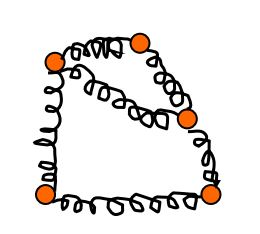
\includegraphics[scale=0.6]{bilder/graphfederfirst}\label{fig_graphfederfirst}
	}
	\hspace{1.0cm}%
	\subfigure[die Federn verschieben die Knoten]
	{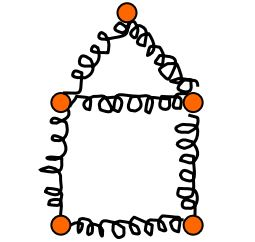
\includegraphics[scale=0.6]{bilder/graphfedersecond}\label{fig_graphfedersecond}
	}
	\hspace{1.0cm}%
	\subfigure[darstellung als Graph]
	{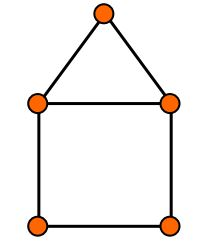
\includegraphics[scale=0.6]{bilder/graphfederthird}\label{fig_graphfederthird}
	}
	\\
	\caption[Darstellung als Stahlkugeln und Federn eines Graphen]{Darstellung als Stahlkugeln und Federn eines Graphen}
	\label{fig_testbild2}
\end{figure}
In diesem Kapitel werden die Grundlagen des Spring-Algorithmus erklärt. 
Es geht um die Verwendung dieser Algorithmen, das grundsätzliche Vorgehen
und die Erweiterbarkeit.


Das Problem der Darstellung basiert auf der Platzierung der Kanten sowie
Knoten um eine möglichst ästhetische Zeichnung des
Graphen zu erhalten, die gut lesbar und verständlich ist. Die grundlegenden Kriterien für eine ästhetischen Zeichnung eines Graphen sind:
\begin{enumerate}
	\item die Knoten sollten gleichmäßig verteilt werden
	\item minimale Überschneidung der Kanten
	\item einheitliche Länge der Kanten
	\item möglichst symmetrisch
	\item alles soll sich innerhalb der Fläche befinden[3].
\end{enumerate}   

Das heißt es ist leicht möglich
die wichtigen Informationen des Graphen anhand einer visuellen Darstellung zu erhalten. 
Dazu gehören unter anderem die Erkennung von Verbindungen zwischen Knoten oder deren Lage. Dies
ist vor allem wichtig bei einer MetroMap wo es darum geht schnell herauszufinden wie es möglich ist
von einem Punkt zu einem anderen zu kommen.
Um dies zu erreichen gibt es verschiedenste Ansätze.

Im Folgenden wird es um ein Verfahren gehen, welches auf ein Modell
der Physik basiert, indem Stahlkugeln für die Knoten, und Federn für die Kanten stehen. Durch die 
Federn wirken Kräfte auf die Kugeln ein, wodurch sich diese verschieben. Dies passiert solange, 
bis die Federn ihre optimale Länge haben. Die optimale Länge $k$ wird durch die Anzahl der Knoten sowie
der zur Verfügung stehender Fläche $A$ bestimmt:

\begin{align}
	k =
	\sqrt{A / |V|}
\end{align}

\begin{align}
	A =
	W * L.
\end{align}

$W$ ist die Weite und $L$ die Länge der zugrunde liegenden Oberfläche, auf der, der Graph gezeichnet wird. Es ist
wichtig zu wissen wie diese Maße sind um eine bessere Verteilung der Knoten zu ermöglichen. 

Bildet die bisherige 
Platzierung der Kanten und Knoten einen planaren Graphen, so wird die neue die Platzierung in fast allen Fällen
auch planar sein. Ein Graph ist planar wenn sich keine Kanten überschneiden, diese Eigenschaft ist besonders gewollt um den resultierenden Graphen noch übersichtlicher zu gestalten.





\section{Spring-Algorithmus - Vorgehen}
\label{Kapitel_3_-_Unterkapitel_2}
%

\begin{algorithm}[t]
	\centering
	\caption[Ein Algorithmus]{Spring-Algorithmus} \label{algo_1}
	\begin{algorithmic}
		\REQUIRE \begin{math} G:= (V,E) \end{math}
		\ENSURE \begin{math} G:= (V,E) \end{math}
		\FOR{\begin{math}i:=1 \leq iterations \end{math}}
		\FOR{\begin{math}v_{i} \in V\end{math}}
		\STATE $d_{v_{i}} := 0;$
		\FOR{(\begin{math}v_{j} \in V\end{math})}
		\IF{$v_{i}\neq v_{j}$}
		\STATE $\Delta := p_{v_{i}} - p_{v_{j}};$
		\STATE $d_{v_{i}} := d_{v_{i}} + (\Delta / |\Delta|) \cdot f^{r}_{v_{i},v_{j}}(|\Delta|));$
		\ENDIF
		\ENDFOR
		\ENDFOR
		\newline
		\FOR{\begin{math}e_{v_{i},v_{j}} \in E\end{math}}
		\STATE $\Delta := p_{v_{i}} - p_{v_{j}};$
		\STATE $d_{v_{i}} := d_{v_{i}} - (\Delta / |\Delta|) \cdot f^{a}_{v_{i},v_{j}}(|\Delta|));$
		\STATE $d_{v_{j}} := d_{v_{j}} + (\Delta / |\Delta|) \cdot f^{a}_{v_{i},v_{j}}(|\Delta|));$
		\ENDFOR
		\newline
		\FOR{\begin{math}v_{i} \in V\end{math}}
		\STATE $p_{v_{i}} := p_{v_{i}} + ( d_{v_{i}}/ |d_{v_{i}}|) \cdot min ( d_{v_{i}}, t );$
		\STATE $p_{v_{i}}^{x} := min(W/2, max(-W/2, p_{v_{i}}^{x}));$
		\STATE $p_{v_{i}}^{y} := min(L/2, max(-L/2, p_{v_{i}}^{y}))$
		\ENDFOR
		\STATE $t:= cool(t)$
		\ENDFOR
	\end{algorithmic}
\end{algorithm}

Zwischen jedem Knotenpaar $v_{i},v_{j} \in V$ wird eine abstoßende Kraft \begin{math} f^{r}_{v_{i},v_{j}}  \end{math} berechnet.   Alle
benachbarten Knoten erhalten eine anziehende Kraft \begin{math} f^{a}_{v_{i},v_{j}} \end{math}. Zwei Knoten \begin{math} v_{i},v_{j} \in V \end{math}sind benachbart wenn \begin{math} e_{v_{i},v_{j}} \in E \end{math} ist. Das führt dazu, dass verbundene Knoten näher zusammen
gezeichnet werden, während sie noch immer einen gewissen Abstand zueinander
haben. Der Algorithmus geht dabei in drei Schritten vor:

\begin{enumerate}
	\item zwischen jedem Knotenpaar die abstoßende Kraft berechnen
	\item benachbarten Knoten eine anziehende Kraft zuweisen
	\item jeden Knoten seiner neuen Kraft nach bewegen.
\end{enumerate} 
Diese drei Schritte werden werden so oft wiederholt bis keine weitere Bewegung mehr stattfindet.
Die Funktionen \begin{math} f^{a}_{v_{i},v_{j}} \end{math} und \begin{math} f^{r}_{v_{i},v_{j}} \end{math} sind wie folgt definiert:


\begin{align}
	f^{a}_{v_{i},v_{j}} (x) =
	x^{2}/k
\end{align}

\begin{align}
	f^{r}_{v_{i},v_{j}} (x) =
	-k^{2}/x.
\end{align}


\begin{figure}[t]
	\centering
	\subfigure[anziehende Kraft $f^{a}$ zwischen dem dritten und vierten Knoten]
	{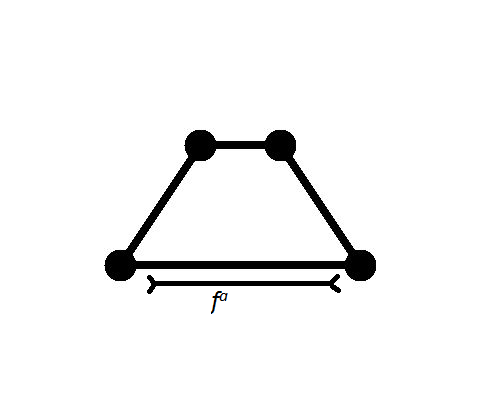
\includegraphics[scale=0.3]{bilder/kraftfa}\label{fig_kraftfa}
	}
	\hspace{1.0cm}%
	\subfigure[abstoßende Kraft $f^{r}$ zwischen dem ersten und vierten Knoten]
	{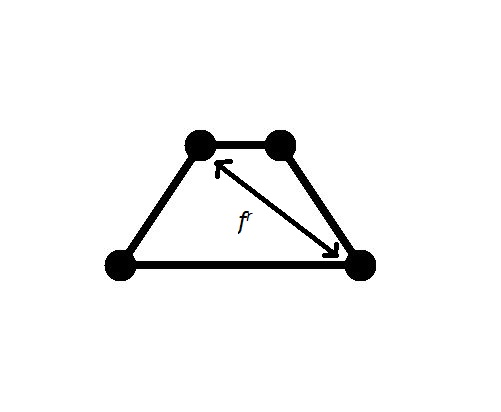
\includegraphics[scale=0.3]{bilder/kraftfr}\label{fig_kraftfr}
	}
	\hspace{1.0cm}%
	\subfigure[die wirkenden Kräfte lösen sich auf]
	{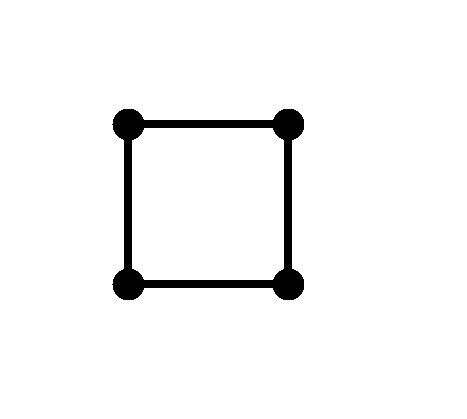
\includegraphics[scale=0.3]{bilder/standardgraph}\label{fig_standardgraph}
	}
	\\
	\caption[Wirkende Kräfte im Graphen]{Wirkende Kräfte im Graphen}
	\label{fig_testbild2}
\end{figure} 


Der Vektor $d_{v_{i}}$ gibt an in welcher Richtung der Knoten $v_{i}$ bewegt wird. Während der Vektor $p_{v_{i}}$ auf die momentane Position des Knoten $v_{i}$ zeigt. Der Vektor $\Delta$ ist die Differenz zwischen $p_{v_{i}}$ und $p_{v_{j}}$, der Richtungsvektor von $v_{i}$ nach $v_{j}$. Die Variable $iterations$ gibt die Anzahl der Durchläufe an. Bei jedem neuen Durchlauf wird der Vektor  $d_{v}$  eines jeden Knotens $v$ auf 0 gesetzt. Mit zwei For-Schleifen geht man jede Knotenkombination durch und berechnet die abstoßende Kraft $f^{r}_{v_{i},v_{j}}$ mithilfe der Länge des $\Delta$ Vektors. Anschließend wird der Bewegungsvektor auf den Einheitsvektor von $\Delta$ multipliziert mit der berechneten Kraft gesetzt. Dadurch drücken sich die Knoten direkt voneinander weg.

Der zweite Schritt besteht darin die anziehenden Kräfte zwischen den benachbarten Knoten zu berechnen. Dazu wird jede Kante einmal durchgegangen und der Bewegungsvektor von jedem betroffenen Knoten wird wie bei der abstoßenden Kraft aufaddiert. 

Im letzten Schritt des Algorithmus werden die Knoten nun in Richtung ihres Bewegungsvektors bewegt. Es wird darauf geachtet, dass die Knoten dabei nicht das Bild verlassen. Die Variable $t$ ermöglicht es, am Anfang viel Bewegung der Knoten zuzulassen und dies immer weiter einzuschränken, damit mit der Graph mit jeder Iteration feiner wird. Die Funktion $cool(t)$ regelt dabei wie weit sich jeder Knoten in der nächsten Iteration maximal bewegen darf. $t$ könnte zum Beispiel bei der Länge des Bildes starten und sich nach jeder Iteration um ein Zehntel mit $cool(t)$ kürzen. Nach 10 Iterationen wären dadurch keine weiteren Bewegungen der Knoten mehr möglich.


\section{Spring-Algorithmus - Erweiterbarkeit}
\label{Kapitel_3_-_Unterkapitel_3}   
Eine besondere Eigenschaft dieses Algorithmus ist die leichte Erweiterbarkeit. Er kann leicht an viele verschiedene Probleme angepasst werden.
Der Algorithmus 2.1 ist bereits eine erste Erweiterung des ursprünglichen Algorithmus. Beim Bewegen der Knoten im dritten Schritt wird sichergestellt, dass sich die Knoten weiterhin auf der zur Verfügung stehenden Fläche befinden.

Ebenfalls modifizierbar sind die Funktionen $f^{a}_{v_{i},v_{j}}$ und $f^{r}_{v_{i},v_{j}}$. Im Kapitel 3 wird dies genutzt um den Graphen weiter anzupassen. Es ist leicht möglich noch weitere Kräfte miteinzubeziehen oder sie ganz anderen Knoten zuzuweisen. Im späteren Verlauf wird es auch Knoten geben, die sich nicht bewegen sollen, weil sie zum Beispiel größere Städte oder zentrale Verbindungspunkte sind.

%